\documentclass[letterpaper,12pt]{article}
\usepackage{tabularx} % extra features for tabular environment
\usepackage{amsmath}  % improve math presentation
\usepackage{graphicx} % takes care of graphic including machinery
\usepackage[margin=1in,letterpaper]{geometry} % decreases margins
\usepackage{cite} % takes care of citations
\usepackage[final]{hyperref} % adds hyper links inside the generated pdf file
\usepackage{color}
\hypersetup{
	colorlinks=true,       % false: boxed links; true: colored links
	linkcolor=blue,        % color of internal links
	citecolor=blue,        % color of links to bibliography
	filecolor=magenta,     % color of file links
	urlcolor=blue
}

\begin{document}

\title{CPEG466 Report}
\author{Ryan Kabrick}
\date{December 8th, 2018}
\maketitle

\begin{abstract}
This semester I have completed several different tasks for CAPSL. Besides helping with administrative duties at the lab, I have successfully configured the software stack of the DEMAC cluster and worked side by side with Diego R. and Jose M. to bring it up and tests its configuration. My contributions to the DEMAC project are manifold, but the most important include installation, configuration and use of Ansible, which allows distribution of commands across the cluster, as well as configuration and testing of MPI on the full 24 node cluster. While there is still countless projects to be completed, this is a summary of my work in the past few months.
\end{abstract}

\section{List of contributions and acquired knowledge}

\begin{itemize}
\item Configuration of the Parallella boards Operating System
\item Configuration of Ansible playbooks for fast deployment of software on the 24 boards cluster
\item Configuration of the MPI compiler and runtime
\item Running the High-Performance Linpack Benchmark for Distributed-Memory Computers in the cluster
\end{itemize}

\section{DEMAC Cluster}
I have spent a majority of my time working on the cluster of Parallella boards. With both Jose and Diego's help. Following I explain each of my contributions and describe the different challenges that I had to face throughout this time.

\subsection{The Parallela Ubuntu}
By using the getting started reference manual \cite{parallellaRefManual}, I loaded the customized version of Ubuntu Linux OS into the Parallella's SD card. There are two different version of this OS. A headless version which has no support for the HDMI port in the board, and a version that provides graphical interface and that could be connected to a screen through the HDMI interface.

My first approach used the Ubuntu version with HDMI support, which reduced the complexity of my learning curve. After getting familiarized with the graphical interface, I trained myself in the use of SSH, and proceeded to use the headless (no HDMI) version of Ubuntu. This required me to understand the client-server model of the SSH connection, as well as the password and password-less connection to the board.

\subsection{Creating the DEMAC linux image 0.1} \label{sec:demac_linux_image}
In addition to the programs that come with the Parallella Ubuntu, our cluster required extra configuration steps that we would like to avoid whenever increasing the number of nodes on our cluster, or replacing a cluster node. For this reason I created a master image for the SD cards which included the necessary programs for the cluster including
  \begin{enumerate}
  \item \textbf{Ansible}: This program uses SSH under the hood to send configuration commands to all the cluster at once. Ansible uses Playbooks and System description files and it provides high flexibility and easy of use. Ansible allows us to automate the configuration of the cluster by sending a single command to all of the nodes at once.
  \item \textbf{IP Configuration}:  Each board should have a single IP and be able to communicate with the others. Given that we do not have a DHCP server configured, it is necessary to statically configure the IP of each node. This step is not possible to completely automatize in the generation of the image, but we provide the file with the configuration that remains the same across all the nodes, while leaving the placeholder IP that allows us to later on change that IP for the particular node.
  \item \textbf{the $/etc/hosts$ file}: By modifying each node's hosts file, we are able to use domain names instead of IP addresses. This makes it easier for the user, to know which node we are referring to.
  \item \textbf{MPICH}: MPI is a programming model that allows the creation of multiple processes across many cluster nodes, and provides the necessary means to allow these processes to communicate across the network. In order to support MPI, an implementation of it is required. MPICH provides the necessary compiler and runtime that allows for the distribution of computation across many different nodes. This requires certain configuration steps which include: 1. password-less ssh connectivity between the nodes. 2. cluster description file with a list of all the possible compute nodes. 3. understanding the MPI Command Line Interface (CLI) options and flags.
  \item \textbf{Attempted NFS configuration}: While MPICH allows the distribution of computation, it relies on an underlying shared file system. This allows the different nodes to be able to start the execution of the running program, and also share the different input files. A large amount of time was spent trying to make NFS work, but these attempts were not successful due to a problem in the way the Linux Kernel is compiled in the Parallella boards (see \cite{parallellaNFSProblem}). For this reason, we are currently relying on manually moving the file across the boards through the use of ansible and a git repository. I understand that this approach is not ideal, but it allowed me to proceed with the execution of the benchmarks.

  \end{enumerate}

\subsection{Git repository}
I have created and maintained the git repository in \cite{demac_git_repo}. This repo holds all of the files regarding the cluster, it also allows easy configuration of the cluster nodes, and in the absence of an NFS solution, we are using it to coordinate file distribution.


\subsection{The HPL Linpack Benchmark}
After multiple conversations with Jose regarding what program to run on the system to be able to test it out we have decided to use the widely adopted HPL Linkpack benchmark. Using this program has allowed me to understand the process of the Top500 supercomputers, which uses a version of this benchmark \cite{top500_linpack}.

To this end I have successfully compiled and tested the HPL linpack benchmark to test the performance of the cluster. We have used the default workload file, and we have started by using exploring strong scalability across the system. While the results were not satisfying for reasons we show in the section \ref{sec:results}, it served as a proof of concept that the cluster is almost ready to start receiving real MPI computation.

\subsection{Documentation}
This project is an extension of my effort during Summer this year. Back then I wrote an initial version of the documentation of the Parallella boards. However, thanks to the acquired knowledge through this semester, I was able to updated and rewrite part of such document. This documentation details the process of getting the cluster to the point it is at now, including the image mentioned in section \ref{sec:demac_linux_image}

\section{Results} \label{sec:results}
The results obtained from the HPL benchmark were confusing the say the least. It appears as though the more processes that MPI distributes the tests do, the slower the overall performance is. There are two peaks at \textbf{12} and \textbf{36} processes which are worth noting. Although we still do not have the data to provide a valuable explanation of this behavior we believe that the current issue is that the size of the problem is still not large enough to show a speedup as the number of cores increases. It is also interesting that 12 is a multiple of 36. Further experimentation and profiling of the execution is required to explain this behavior.

\begin{figure}[h]
  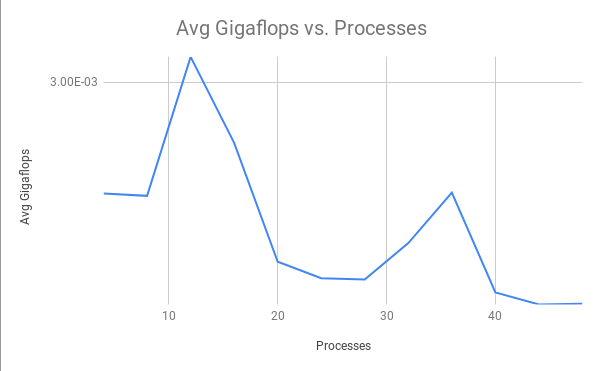
\includegraphics[width = \linewidth]{avgGig.png}
  \caption{Average $\frac{Gigaflop}{Second}$ vs. Number of Processes} \label{fig:avgGig}
  \end{figure}
From figure \ref{fig:avgGig} it can be assumed that the workload was not significant to warrant an increase in overall performance. It appears that the overall performance is decreased the more the computation is distributed. I believe this is due to the fact that more processes corresponds to more time spent communicating between nodes. This leads me to believe a more complex workload will make the communication time less impactful to the overall performance results.

\begin{figure}[h]
  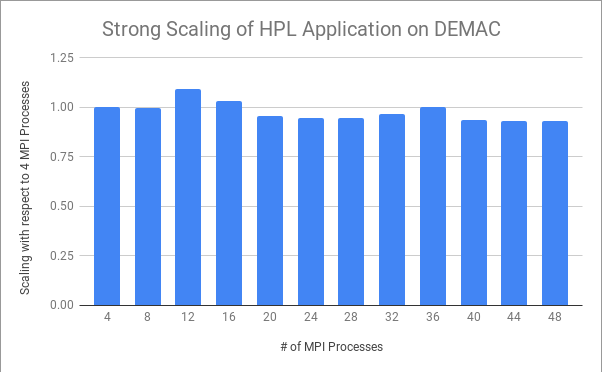
\includegraphics[width = \linewidth]{strongScaling.png}
  \caption{Strong Scaling}\label{fig:strongScale}
\end{figure}

From figure \ref{fig:strongScale} uses as baseline the result for 4 nodes. This allows us to compare the execution time to a common base time, and explore and understand the concept of strong scaling. The question this graph answers is what is the effect on the execution time as the number of processes increases, and it compliments our finding of figure \ref{fig:avgGig}.

\section{Auxiliary Tasks}
In addition to working on the cluster, I have also completed a few tasks around the lab room including:
\begin{itemize}
\item Replacing the old printer
\item Sorting through, documenting, and removing duplicates from Dr. Gao's library
\item Use Latex to generate this report.
\item {\color{red}I'll fill this in later}
\end{itemize}

\section{Future Work}

    There is still much to be done in the future with the cluster specifically. The Parallella has both an dual-core ARM processor as well as the 16-core Epiphany coprocessor. As of now, MPI on the parallelas can only split computation between all the nodes using the two cores on the ARM processor on each node. This means that all of the power of the Epiphany coprocessor is not being utilized. To truly exploit the potential of this parallel cluster, I would like the opportunity to explore the Epiphany Software Development Kit (eSDK) that exposes the API for programming the epiphany chip, and see how it would be possible to combine MPI to use the full power of the Parallella boards and the DEMAC cluster. My goal for the end of Winter session is to successfully run a program with MPI that exploits the Epiphany chip.

In order to achieve this, I propose to start with an already existing MPI benchmark, profile to identify the hot regions of code that consume the most, and then create an implementation on the epiphany chip using the eSDK. This will allow me to explore scalability of an application across the cluster, and also get familiarized with the programming model on the parallella board.

\bibliography{Ryan}
\bibliographystyle{ieeetr}

\end{document}
